\documentclass[aspectratio=169,10pt]{beamer}
\usetheme{default}
\usepackage[utf8]{inputenc}
\usepackage[T1]{fontenc}
\usepackage{libertinus}
\usepackage[none]{hyphenat}
\hyphenpenalty=10000\exhyphenpenalty=10000
\usepackage{xcolor}
\usepackage{hyperref}
\usepackage{tikz}
\usetikzlibrary{shapes.geometric, arrows.meta, positioning, shadows}

\definecolor{navy}{HTML}{0F2A44}
\definecolor{navydeep}{HTML}{0A1C30}
\definecolor{teal}{HTML}{0E7C6B}
\definecolor{teallight}{HTML}{DDF0EB}
\definecolor{accent}{HTML}{F2A541}
\definecolor{light}{HTML}{F2F5F7}
\definecolor{accentdeep}{HTML}{C77F1F}
\definecolor{cardbd}{HTML}{D7E3E0}
\definecolor{muted}{HTML}{5B6B7A}
\definecolor{warnbg}{HTML}{FFF4E0}
\definecolor{stepbd}{HTML}{B9D6CF}

\setbeamercolor{structure}{fg=navy}
\setbeamercolor{frametitle}{fg=navy}
\setbeamertemplate{navigation symbols}{}
\setbeamertemplate{footline}{%
  \hfill\textcolor{muted}{\scriptsize PreClaim Guard \textbar{} Healthkathon 2026 \textbar{} \insertframenumber}\hspace{0.4cm}\vspace{0.2cm}%
}
\setbeamertemplate{frametitle}{%
  \vspace{0.25cm}\hspace{0.4cm}{\Large\bfseries\insertframetitle}\par\vspace{0.12cm}%
}

% stat card: #1 big number, #2 desc, #3 source
\newcommand{\statcard}[3]{%
  \begin{tikzpicture}
    \node[rounded corners=4pt, fill=navy, minimum width=3.75cm, minimum height=2.7cm, inner sep=0pt, drop shadow={opacity=0.18}] (box) {};
    \node[anchor=north west, text=accent, font=\Large\bfseries] at ([xshift=7pt,yshift=-5pt]box.north west) {#1};
    \node[anchor=north west, text=white, font=\scriptsize, text width=3.3cm] at ([xshift=7pt,yshift=-28pt]box.north west) {#2};
    \node[anchor=south west, text=white!55, font=\tiny, text width=3.3cm] at ([xshift=7pt,yshift=5pt]box.south west) {\textit{#3}};
  \end{tikzpicture}%
}
% info card: #1 title, #2 body, #3 footer
\newcommand{\infocard}[3]{%
  \begin{tikzpicture}
    \node[rounded corners=4pt, fill=white, draw=cardbd, line width=0.7pt, minimum width=3.75cm, minimum height=2.25cm, inner sep=0pt] (box) {};
    \node[anchor=north west, text=teal, font=\small\bfseries] at ([xshift=7pt,yshift=-5pt]box.north west) {#1};
    \node[anchor=north west, text=navy!80, font=\scriptsize, text width=3.3cm] at ([xshift=7pt,yshift=-20pt]box.north west) {#2};
    \node[anchor=south west, text=muted, font=\tiny, text width=3.3cm] at ([xshift=7pt,yshift=5pt]box.south west) {#3};
  \end{tikzpicture}%
}
% half card (wider): #1 title, #2 body
\newcommand{\halfcard}[2]{%
  \begin{tikzpicture}
    \node[rounded corners=4pt, fill=white, draw=cardbd, line width=0.7pt, minimum width=5.7cm, minimum height=2.0cm, inner sep=0pt] (box) {};
    \node[anchor=north west, text=teal, font=\small\bfseries] at ([xshift=8pt,yshift=-6pt]box.north west) {#1};
    \node[anchor=north west, text=navy!80, font=\scriptsize, text width=5.25cm] at ([xshift=8pt,yshift=-21pt]box.north west) {#2};
  \end{tikzpicture}%
}
% step box for roadmap: #1 label, #2 body
\newcommand{\stepbox}[2]{%
  \begin{tikzpicture}
    \node[rounded corners=4pt, fill=teallight, draw=stepbd, line width=0.6pt, minimum width=2.8cm, minimum height=2.1cm, inner sep=0pt] (box) {};
    \node[anchor=north west, text=teal, font=\scriptsize\bfseries] at ([xshift=6pt,yshift=-5pt]box.north west) {#1};
    \node[anchor=north west, text=navy!85, font=\scriptsize, text width=2.5cm] at ([xshift=6pt,yshift=-19pt]box.north west) {#2};
  \end{tikzpicture}%
}

\begin{document}

% ---- Slide 1: Cover ----
{\setbeamercolor{background canvas}{bg=navydeep}
\begin{frame}[plain]
\begin{tikzpicture}[remember picture, overlay]
  \fill[teal, opacity=0.16] (current page.north east) circle [radius=4.2cm];
  \fill[accent, opacity=0.10] ([xshift=-1cm,yshift=1cm]current page.south west) circle [radius=3.0cm];
\end{tikzpicture}
\vspace{0.45cm}
\hspace{0.35cm}{\scriptsize\color{accent}\MakeUppercase{BPJS Kesehatan --- Healthkathon 2026}}\par
\vspace{0.1cm}
\hspace{0.35cm}{\Huge\bfseries\color{white} PreClaim Guard\par}
\vspace{0.14cm}
\hspace{0.35cm}{\color{white!88} Evidence-Grounded, Policy-Aware, Local-First\par}
\hspace{0.35cm}{\color{white!88} Pre-Claim Compliance Assistant untuk Koder JKN\par}
\vspace{0.2cm}
\hspace{0.35cm}{\Large\itshape\color{accent} Detect before submit. Explain before reject.\par}
\vspace{0.28cm}
\hspace{0.35cm}{\small\color{white!80} Faskes Risk \textbar{} Upcoding \textbar{} Unbundling \textbar{} Cloning \& Repeat Billing\par}
\vspace{0.14cm}
\hspace{0.35cm}{\small\color{white!65} Tim ProfHabibieBanggaSamaKita\par}
\hspace{0.35cm}{\small\color{white!65} Fatih Jawwad Al Mumtaz (Ketua) \textbar{} Farrel Ghozy Affifuddin (Anggota)\par}
\vspace{0.35cm}
\end{frame}
}

% ---- Slide 2: Positioning ----
\begin{frame}{Quality gate sebelum klaim keluar dari RS}
{\small\color{navy!80} Satu kategori: \textbf{Efisiensi Risiko Faskes}. Fokus: \textbf{Upcoding}, \textbf{Unbundling}, \textbf{Cloning/Repeat Billing}. Verifikasi BPJS represif setelah klaim masuk --- kami preventif sebelum keluar.\par}
\vspace{0.22cm}
\begin{columns}[T,onlytextwidth]
\column{0.32\textwidth}\centering
\infocard{Sebelum submit}{Rule + evidence check di meja koder, temuan beralasan + versi aturan.}{Bukan vonis fraud}
\column{0.32\textwidth}\centering
\infocard{Human-in-the-loop}{Keputusan akhir di koder: perbaiki atau setujui dengan catatan.}{Tak ada tolak otomatis}
\column{0.32\textwidth}\centering
\infocard{Local-first}{Data pasien tak keluar RS; prototype murni synthetic.}{UU PDP No.\ 27/2022}
\end{columns}
\end{frame}

% ---- Slide 3: Masalah skala nasional ----
\begin{frame}{Uang tertahan triliunan, fraud-nya nyata}
\begin{columns}[T,onlytextwidth]
\column{0.32\textwidth}\centering
\statcard{Rp5,92 T}{Klaim ditunda BPJS akhir 2024 atas 3,69 jt kasus.}{Bisnis.com, Mei 2025}
\column{0.32\textwidth}\centering
\statcard{Rp34 M}{Fraud 3 RS via \mbox{phantom billing}; KPK menindak.}{KPK, Jul 2024}
\column{0.32\textwidth}\centering
\statcard{3 RS}{Upcoding + phantom billing naik ke penyidikan.}{Kejari Jember, Mei 2026}
\end{columns}
\vspace{0.18cm}
\hspace{0.2cm}{\small\itshape\color{muted} 284 jt peserta JKN aktif (Jul 2026) --- program tunggal terbesar di dunia. Tiap perbaikan klaim berdampak sistemik.\par}
\end{frame}

% ---- Slide 4: Bukti RS (full-slide chart) ----
\begin{frame}{Pending kecil berkas, besar nilai --- RSUD Pasar Minggu 2024}
\begin{center}
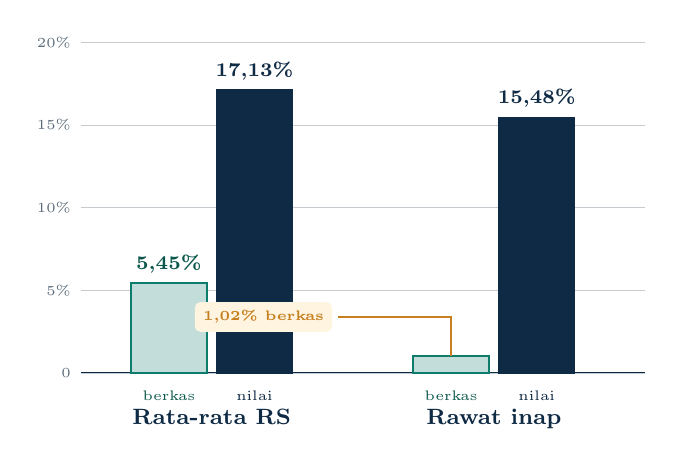
\begin{tikzpicture}[y=0.21cm, x=1.28cm, font=\scriptsize]
  % axes + baseline
  \draw[color=navy, line width=0.6pt] (0,0) -- (5.6,0);
  \foreach \y/\lbl in {0/0, 5/5\%, 10/10\%, 15/15\%, 20/20\%} {
    \draw[color=muted!35] (0,\y) -- (5.6,\y);
    \node[left, color=muted, font=\tiny] at (0,\y) {\lbl};
  }
  % GROUP A: rata-rata
  \fill[teal!25, draw=teal, line width=0.7pt] (0.5,0) rectangle (1.25,5.45);
  \fill[navy, draw=navy] (1.35,0) rectangle (2.10,17.13);
  \node[above, font=\scriptsize\bfseries, text=teal!70!black] at (0.875,5.45) {5,45\%};
  \node[above, font=\scriptsize\bfseries, text=navy] at (1.725,17.13) {17,13\%};
  \node[below, font=\tiny, text=teal!70!black] at (0.875,-0.5) {berkas};
  \node[below, font=\tiny, text=navy] at (1.725,-0.5) {nilai};
  \node[below, font=\footnotesize\bfseries, text=navy] at (1.30,-1.6) {Rata-rata RS};
  % GROUP B: ranap
  \fill[teal!25, draw=teal, line width=0.7pt] (3.30,0) rectangle (4.05,1.02);
  \fill[navy, draw=navy] (4.15,0) rectangle (4.90,15.48);
  \node[above, font=\scriptsize\bfseries, text=navy] at (4.525,15.48) {15,48\%};
  \node[below, font=\tiny, text=teal!70!black] at (3.675,-0.5) {berkas};
  \node[below, font=\tiny, text=navy] at (4.525,-0.5) {nilai};
  \node[below, font=\footnotesize\bfseries, text=navy] at (4.10,-1.6) {Rawat inap};
  % callout for tiny bar
  \draw[color=accentdeep, line width=0.6pt] (3.675,1.02) -- (3.675,3.4) -- (2.55,3.4);
  \node[anchor=east, font=\tiny\bfseries, text=accentdeep, fill=warnbg, rounded corners=2pt, inner sep=3pt] at (2.50,3.4) {1,02\% berkas};
\end{tikzpicture}
\end{center}
\vspace{0.05cm}
{\scriptsize\color{muted} \tikz{\fill[teal!25,draw=teal] (0,0) rectangle (0.3,0.2);} \% berkas (jumlah) \quad \tikz{\fill[navy] (0,0) rectangle (0.3,0.2);} \% nilai (rupiah) \quad \textbar{} \quad Sumber: Wirdah dkk., COMSERVA 5(2), 2025.\par}
\vspace{0.05cm}
{\small\color{navy} \textbf{Baca:} 1,02\% berkas ranap menahan 15,48\% nilai --- coding dominan dari sisi nilai. Aturan berversi + kalibrasi lokal.\par}
\end{frame}

% ---- Slide 5: Solusi ----
\begin{frame}{Tiga lapis pemeriksaan, satu keputusan di koder}
\begin{center}
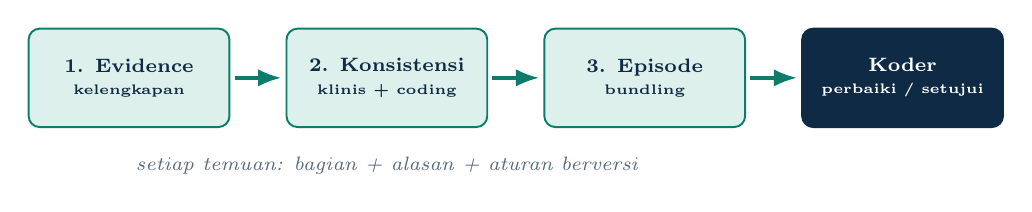
\begin{tikzpicture}[node distance=7mm,
  stage/.style={rounded corners=4pt, fill=teallight, draw=teal, line width=0.7pt, minimum width=2.55cm, minimum height=1.25cm, font=\scriptsize\bfseries, text=navy, align=center},
  arr/.style={-Latex, line width=1.2pt, color=teal, shorten >=1.5pt, shorten <=1.5pt}]
  \node[stage] (a) {1. Evidence\\{\tiny kelengkapan}};
  \node[stage, right=of a] (b) {2. Konsistensi\\{\tiny klinis + coding}};
  \node[stage, right=of b] (c) {3. Episode\\{\tiny bundling}};
  \node[stage, fill=navy, draw=navy, text=white, right=of c] (d) {Koder\\{\tiny perbaiki / setujui}};
  \draw[arr] (a) -- (b); \draw[arr] (b) -- (c); \draw[arr] (c) -- (d);
  \node[below=2.5mm of b, text=navy!70, font=\scriptsize\itshape] {setiap temuan: bagian + alasan + aturan berversi};
\end{tikzpicture}
\end{center}
\vspace{0.1cm}
\begin{columns}[T,onlytextwidth]
\column{0.48\textwidth}\centering
\halfcard{Temuan beralasan}{Severity + bahasa manusia + evidence pemicu + rule ID/versi/sumber. Confidence terpisah dari skor.}
\column{0.48\textwidth}\centering
\halfcard{Re-check menutup loop}{Setelah koreksi / persetujuan beralasan, cek ulang + audit tampilkan yang berubah.}
\end{columns}
\end{frame}

% ---- Slide 6: Diferensiasi ----
\begin{frame}{Arena faskes kosong dari juara bertahan}
{\small\color{navy!80} Juara 2025 semua di sisi peserta + preventive care --- tak satu pun menyentuh fraud faskes. Tema 2026 dipaksa ke efisiensi risiko.\par}
\vspace{0.2cm}
\begin{columns}[T,onlytextwidth]
\column{0.48\textwidth}\centering
\halfcard{Mereka (2025)}{Teman Ibu (Aruna, J1) --- ibu hamil. Lucky Seven (J2) --- jantung. Go Fit 360 (J3) --- kebugaran.}
\column{0.48\textwidth}\centering
\halfcard{Kami (2026)}{Quality gate di meja koder sebelum submit. Komplementer verifikasi BPJS, bukan pengganti.}
\end{columns}
\vspace{0.14cm}
\hspace{0.2cm}{\tiny\color{muted} Sumber: Detik/Tempo/Kompas/CNN Indonesia, Nov 2025.\par}
\end{frame}

% ---- Slide 7: Teknis ----
\begin{frame}{Klaim masuk, temuan beralasan keluar}
\begin{center}
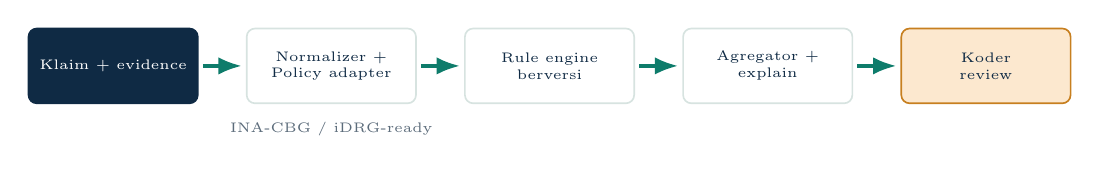
\begin{tikzpicture}[node distance=6mm,
  box/.style={rounded corners=3pt, fill=white, draw=cardbd, line width=0.6pt, minimum width=2.15cm, minimum height=0.95cm, font=\tiny, text=navy, align=center},
  arr/.style={-Latex, line width=1.2pt, color=teal, shorten >=1.5pt, shorten <=1.5pt}]
  \node[box, fill=navy, draw=navy, text=white] (i) {Klaim + evidence};
  \node[box, right=of i] (n) {Normalizer +\\Policy adapter};
  \node[box, right=of n] (r) {Rule engine\\berversi};
  \node[box, right=of r] (g) {Agregator +\\explain};
  \node[box, fill=accent!25, draw=accentdeep, right=of g] (u) {Koder\\review};
  \draw[arr] (i) -- (n); \draw[arr] (n) -- (r); \draw[arr] (r) -- (g); \draw[arr] (g) -- (u);
  \node[below=1mm of n, text=muted, font=\tiny] {INA-CBG / iDRG-ready};
\end{tikzpicture}
\end{center}
\vspace{0.12cm}
\begin{columns}[T,onlytextwidth]
\column{0.48\textwidth}\centering
\halfcard{Tanpa data JKN riil}{Validasi: agregat publik. Prototype: synthetic + anomali disuntik + kunci jawaban. Pilot: data RS pasca-izin (di luar scope).}
\column{0.48\textwidth}\centering
\halfcard{Stack lokal}{Next.js, FastAPI, PostgreSQL, rules JSON/YAML, scikit-learn, Docker. Target rule path $\leq$1 dtk/klaim.}
\end{columns}
\end{frame}

% ---- Slide 8: Kematangan ----
\begin{frame}{Titik berangkat: blueprint siap dibangun}
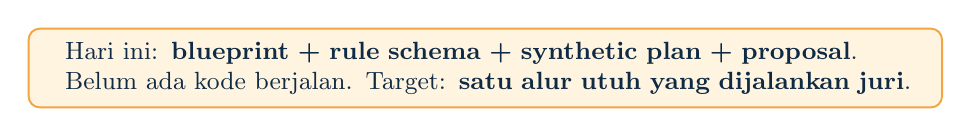
\begin{tikzpicture}
  \node[rounded corners=4pt, fill=warnbg, draw=accent, line width=0.7pt, minimum width=11.6cm, minimum height=1.0cm, inner sep=0pt] (band) {};
  \node[anchor=west, text=navy, font=\small, text width=10.9cm] at ([xshift=10pt]band.west) {Hari ini: \textbf{blueprint + rule schema + synthetic plan + proposal}. Belum ada kode berjalan. Target: \textbf{satu alur utuh yang dijalankan juri}.};
\end{tikzpicture}
\vspace{0.2cm}
\begin{columns}[T,onlytextwidth]
\column{0.48\textwidth}\centering
\halfcard{Sudah ada}{Arsitektur konseptual, ruleset berversi, remediation workflow, synthetic schema, API contract, evidence bank.}
\column{0.48\textwidth}\centering
\halfcard{Target demo terukur}{Unit test 100\%; F1 $\geq$0,75/anomali; FP $<$10\%; 100\% temuan beralasan. Semua pada synthetic.}
\end{columns}
\end{frame}

% ---- Slide 9: Rencana ----
\begin{frame}{Tiga minggu menuju alur utuh}
\begin{columns}[T,onlytextwidth]
\column{0.24\textwidth}\centering
\stepbox{Pra-hackathon}{Problem, schema, synthetic plan, wireframe, repo.}
\column{0.24\textwidth}\centering
\stepbox{Minggu 1}{Generator, rule/evidence engine, dashboard.}
\column{0.24\textwidth}\centering
\stepbox{Minggu 2}{Risk/readiness, remediation, audit, ML baseline.}
\column{0.24\textwidth}\centering
\stepbox{Minggu 3}{Evaluation, security demo, 3 cases, pitch.}
\end{columns}
\vspace{0.18cm}
\hspace{0.2cm}{\small\color{navy!80} Butuh: 2 orang + dokumen aturan resmi + mesin Docker lokal. Pasca: adapter SIMRS/RME, E-Klaim, FHIR/SATUSEHAT --- quality-control layer, bukan pengganti.\par}
\end{frame}

% ---- Slide 10: Dampak ----
\begin{frame}{Lebih banyak masalah selesai sebelum submit}
\hspace{0.2cm}{\small\color{navy} \textbf{Model:} Resolved = Total klaim $\times$ baseline issue $\times$ addressable $\times$ detection $\times$ adoption. Rupiah tak diekstrapolasi nasional.\par}
\vspace{0.2cm}
\begin{columns}[T,onlytextwidth]
\column{0.32\textwidth}\centering
\infocard{RS}{Kasir tak ketahan pending cegah-able; staf tak kerja dua kali.}{Arus kas}
\column{0.32\textwidth}\centering
\infocard{BPJS}{Verifikator tak mengulang salah hulu; beban tepat sasaran.}{Efisiensi}
\column{0.32\textwidth}\centering
\infocard{Sistem}{Integritas JKN; 284 jt peserta terlindungi.}{Kepercayaan}
\end{columns}
\end{frame}

% ---- Slide 11: Risiko ----
\begin{frame}{Patuh dulu: privasi, bias, aturan}
\hspace{0.2cm}{\small\color{navy} \textbf{UU PDP 27/2022:} RS pengendali + pemroses. Lokal di RS, tanpa AI publik di core path. Minimisasi, RBAC, enkripsi, audit, retensi. Synthetic/anonymized saja.\par}
\vspace{0.2cm}
\begin{columns}[T,onlytextwidth]
\column{0.32\textwidth}\centering
\infocard{False positive}{Confidence + threshold + override + feedback.}{100\% beralasan}
\column{0.32\textwidth}\centering
\infocard{Automation bias}{Wording ``needs review''; manusia memutuskan.}{Tanpa vonis}
\column{0.32\textwidth}\centering
\infocard{Aturan basi}{Version + effective date + test + domain review.}{INA-CBG/iDRG}
\end{columns}
\end{frame}

% ---- Slide 12: Tim ----
\begin{frame}{Anggota tim}
\begin{columns}[T,onlytextwidth]
\column{0.48\textwidth}\centering
\halfcard{Fatih Jawwad Al Mumtaz (ketua)}{ML + backend: rule engine, anomali, evaluasi. Kontributor Burn (Rust DL framework); riset edge ML + kuantisasi.}
\column{0.48\textwidth}\centering
\halfcard{Farrel Ghozy Affifuddin (anggota)}{Fullstack + UX: dashboard koder, remediation flow, demo yang bisa dipakai manusia.}
\end{columns}
\vspace{0.18cm}
\hspace{0.2cm}{\small\color{muted} Peran dirangkap (aturan 1--3 orang). Domain reviewer klinis/koding sebagai advisor bila tersedia.\par}
\end{frame}

% ---- Slide 13: Mockup dashboard (full-slide visual) ----
\begin{frame}{Layar koder: antrean, temuan, aksi}
\begin{center}
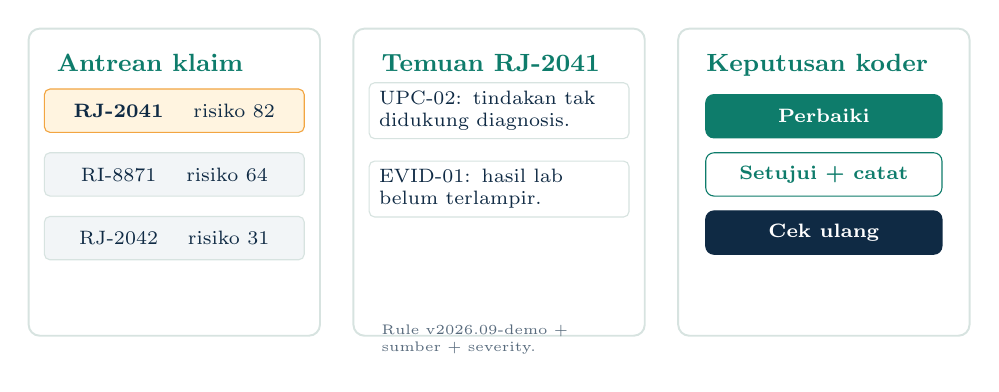
\begin{tikzpicture}[font=\scriptsize,
  panel/.style={rounded corners=4pt, fill=white, draw=cardbd, line width=0.7pt, minimum width=3.7cm, minimum height=3.9cm, inner sep=0pt},
  row/.style={rounded corners=2pt, minimum width=3.3cm, minimum height=0.55cm, inner sep=3pt, font=\scriptsize, align=left},
  btn/.style={rounded corners=3pt, minimum width=3.0cm, minimum height=0.55cm, font=\scriptsize\bfseries, align=center}]
  % panel 1: queue
  \node[panel] (p1) {};
  \node[anchor=north west, text=teal, font=\small\bfseries] at ([xshift=7pt,yshift=-6pt]p1.north west) {Antrean klaim};
  \node[row, fill=warnbg, draw=accent, text=navy] (r1) at ([yshift=-30pt]p1.north) {\textbf{RJ-2041} ~~ risiko 82};
  \node[row, fill=light, draw=cardbd, text=navy] (r2) at ([yshift=-15pt]r1.south) {RI-8871 ~~ risiko 64};
  \node[row, fill=light, draw=cardbd, text=navy] (r3) at ([yshift=-15pt]r2.south) {RJ-2042 ~~ risiko 31};
  % panel 2: finding
  \node[panel, right=4mm of p1] (p2) {};
  \node[anchor=north west, text=teal, font=\small\bfseries] at ([xshift=7pt,yshift=-6pt]p2.north west) {Temuan RJ-2041};
  \node[row, fill=white, draw=cardbd, text=navy, text width=3.05cm] (f1) at ([yshift=-30pt]p2.north) {UPC-02: tindakan tak didukung diagnosis.};
  \node[row, fill=white, draw=cardbd, text=navy, text width=3.05cm] (f2) at ([yshift=-18pt]f1.south) {EVID-01: hasil lab belum terlampir.};
  \node[anchor=north west, text=navy!70, font=\tiny, text width=3.2cm] at ([xshift=7pt,yshift=-104pt]p2.north west) {Rule v2026.09-demo + sumber + severity.};
  % panel 3: action
  \node[panel, right=4mm of p2] (p3) {};
  \node[anchor=north west, text=teal, font=\small\bfseries] at ([xshift=7pt,yshift=-6pt]p3.north west) {Keputusan koder};
  \node[btn, fill=teal, draw=teal, text=white] (b1) at ([yshift=-32pt]p3.north) {Perbaiki};
  \node[btn, fill=white, draw=teal, text=teal] (b2) at ([yshift=-13pt]b1.south) {Setujui + catat};
  \node[btn, fill=navy, draw=navy, text=white] (b3) at ([yshift=-13pt]b2.south) {Cek ulang};
\end{tikzpicture}
\end{center}
\vspace{0.08cm}
{\small\color{navy} Satu layar tanpa pindah aplikasi. Keputusan selalu di manusia; sistem tak menolak otomatis.\par}
\end{frame}

% ---- Slide 14: Storyboard demo (full-slide visual) ----
\begin{frame}{Demo 3 menit: skor turun, kesiapan naik}
\begin{center}
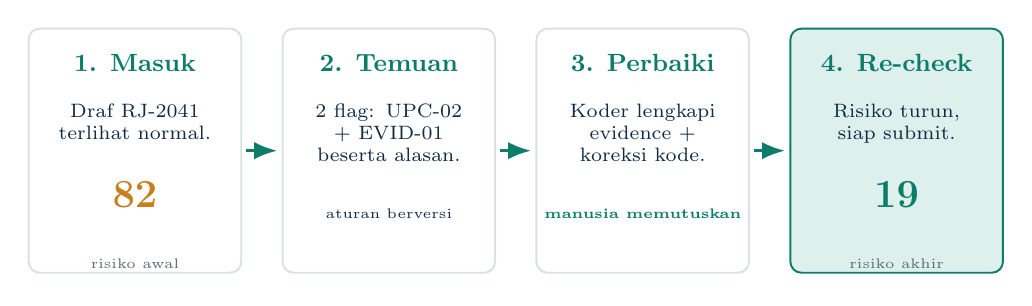
\begin{tikzpicture}[font=\scriptsize,
  demostep/.style={rounded corners=4pt, fill=white, draw=cardbd, line width=0.7pt, minimum width=2.7cm, minimum height=3.1cm, inner sep=0pt},
  arr/.style={-Latex, line width=1.2pt, color=teal, shorten >=1.5pt, shorten <=1.5pt}]
  \node[demostep] (d1) {};
  \node[anchor=north, text=teal, font=\small\bfseries] at ([yshift=-6pt]d1.north) {1. Masuk};
  \node[anchor=north, text=navy, font=\scriptsize, align=center, text width=2.4cm] at ([yshift=-24pt]d1.north) {Draf RJ-2041 terlihat normal.};
  \node[anchor=north, text=accentdeep, font=\Large\bfseries] at ([yshift=-52pt]d1.north) {82};
  \node[anchor=north, text=muted, font=\tiny] at ([yshift=-80pt]d1.north) {risiko awal};
  \node[demostep, right=5mm of d1] (d2) {};
  \node[anchor=north, text=teal, font=\small\bfseries] at ([yshift=-6pt]d2.north) {2. Temuan};
  \node[anchor=north, text=navy, font=\scriptsize, align=center, text width=2.4cm] at ([yshift=-24pt]d2.north) {2 flag: UPC-02 + EVID-01 beserta alasan.};
  \node[anchor=north, text=navy, font=\tiny] at ([yshift=-62pt]d2.north) {aturan berversi};
  \node[demostep, right=5mm of d2] (d3) {};
  \node[anchor=north, text=teal, font=\small\bfseries] at ([yshift=-6pt]d3.north) {3. Perbaiki};
  \node[anchor=north, text=navy, font=\scriptsize, align=center, text width=2.4cm] at ([yshift=-24pt]d3.north) {Koder lengkapi evidence + koreksi kode.};
  \node[anchor=north, text=teal, font=\tiny\bfseries] at ([yshift=-62pt]d3.north) {manusia memutuskan};
  \node[demostep, right=5mm of d3, fill=teallight, draw=teal] (d4) {};
  \node[anchor=north, text=teal, font=\small\bfseries] at ([yshift=-6pt]d4.north) {4. Re-check};
  \node[anchor=north, text=navy, font=\scriptsize, align=center, text width=2.4cm] at ([yshift=-24pt]d4.north) {Risiko turun, siap submit.};
  \node[anchor=north, text=teal, font=\Large\bfseries] at ([yshift=-52pt]d4.north) {19};
  \node[anchor=north, text=muted, font=\tiny] at ([yshift=-80pt]d4.north) {risiko akhir};
  \draw[arr] (d1) -- (d2); \draw[arr] (d2) -- (d3); \draw[arr] (d3) -- (d4);
\end{tikzpicture}
\end{center}
\vspace{0.08cm}
{\small\color{navy} Kesiapan 31 $\rightarrow$ 91. Semua angka synthetic; alur utuh terverifikasi dari input sampai keputusan.\par}
\end{frame}

\end{document}
